\graphicspath{{chapt_dutch/}{intro/}{chapt2/}{chapt3/}{chapt4/}{chapt5/}}

% Header
\renewcommand\evenpagerightmark{{\scshape\small Chapter 4}}
\renewcommand\oddpageleftmark{{\scshape\small Event Simulation and Reconstruction}}

\hyphenation{}

\chapter{Event Simulation and Reconstruction}
\label{ch4}

In order to use the recorded data, the obtained signals coming from various parts of the detector must be reconstructed to be able to identify the particles in the event. Additionally, to compare the experimental results with theory, events are generated and the resulting signals in the detector are simulated, as detailed in Sections~\ref{sec:generation} and \ref{sec:sim}, respectively. The event reconstruction is detailed in Section~\ref{sec:reconstruction}. Finally, some details about the simulation of \acp{SIMP} are given in Section~\ref{sec:SIMPs}.

\section{Event generation}
\label{sec:generation}

% simps -> feynrules -> madgraph
% matching?
% meer detail? Fabio, MCnet school

The event structure at the \ac{LHC} is complicated by the composite nature of protons, as well as the attainable high momentum transfers. A number of aspects must therefore be taken into account when generating events, such as \acp{PDF}, hard scattering, the parton shower, hadronization, and additional activity in the event.

Two partons, meaning the quark or gluon constituents of the colliding protons, will interact with a certain probability for a given momentum transfer. This is parametrized by the \acp{PDF} $f(x, Q^2)$, were $x$ is the momentum fraction of the partons and $Q^2$ is the momentum transfer scale. Experimentally determined \acp{PDF} are available from various groups, including e.g. CTEQ~\cite{Pumplin:2002vw}, MRST/MSTW~\cite{}, and NNPDF~\cite{}. These \acp{PDF} are then used to calculate the matrix element of the hard scattering, which is the process of interest where the two colliding partons create high-energetic final state particles. This is done using an event generator, such as \textsc{MadGraph5\_}a\textsc{MC@NLO} ~\cite{Alwall:2014hca} and \textsc{PowHeg}~\cite{}. With \textsc{MadGraph5\_}a\textsc{MC@NLO} the matrix element can be calculated analytically at tree-level or \ac{LO}, and now at \ac{NLO} as well. This generator was used to generate most of the background processes for the Monojet analysis detailed in Chapter~\ref{ch:monojet} and for the \ac{SIMP} signal used in Chapter~\ref{ch:SIMPs}. \textsc{PowHeg} is able to generate events using \ac{NLO} computations, but only for a relatively limited number of physics processes. In this thesis, background processes from single-top production were generated with this program. Since \ac{NLO} calculations are more time-consuming, one can also scale a \ac{LO} cross section to the \ac{NLO} level by using a so-called k-factor, defined as the ratio of the \ac{NLO} and \ac{LO} cross sections. However, these k-factors often need to be determined as a function of the relevant kinematic variables as they depend on the kinematic phase space and the probed energy scale.

Since the colliding partons have a color charge, the hard scattering will be accompanied by a cascade of radiation from \acs{QCD} processes. This radiation can originate from the incoming partons, which is referred to as \ac{ISR}, or the outgoing partons in the final state, the so-called \ac{FSR}. The perturbative evolution of the cascade can be modeled using the DGLAP (Dokshitzer-Gribov-Lipatov-Altarelli-Parisi) equations~\cite{}. These equations describe the time evolution of the probability of a `mother' parton to split into `daughter' partons at an energy scale $Q^2$. The momentum of the mother is then divided among the daughter partons, which can in turn split into other partons at a lower $Q^2$ scale. The cascade continues down to an energy scale $\Lambda_{QCD}$ where the strong coupling constant becomes unity.

The next step after the showering is the hadronization of the colored particles produced in the parton shower, transforming them into color-neutral hadrons. Since this happens at low energy scales where the perturbative approach of \acs{QCD} is not valid, phenomenological models have to be used. For most of the processes considered in this thesis, the showering and hadronization is done with \textsc{Pythia 8}~\cite{Sjostrand:2006za}, using a standard set of parameters which were tuned to reproduce the experimental data. 

In addition to \ac{ISR} and \ac{FSR}, also beam remnants and multiple parton interactions give rise to additional activity in the event, referred to as the underlying event. After the partons participating in the hard scattering are extracted, the remainder of the protons have a non-zero color charge. The creation of additional hadrons during the hadronization is therefore possible. Multiple parton interactions represent additional interactions which can take place between other incoming partons. Finally, additional collisions between other protons in the same bunch crossing or from a previous bunch crossing, respectively referred to as in-time and out-of-time pileup, add extra activity in the event.

\section{Detector simulation}
\label{sec:sim}

% Delphes?

After being generated, the collision events are passed on to the \ac{CMS} detector simulation, which is based on the \textsc{Geant 4}~\cite{} simulation toolkit. This toolkit provides a description of the interaction between particles and the detector material, including effects such as bremsstrahlung of charged particles, photon conversions, energy loss of charged particles by ionization, and the showering of electrons, photons and hadrons in the calorimeters due to interaction with the material. The \ac{CMS} simulation package contains the geometry of the detector with all the sensitive layers designed to detect the traversing particles, as well as the dead material regions consisting of e.g. support structures, cables and cooling pipes. A precise map of the magnetic field is also included in order to simulate the curvature of the charged particles correctly.

Next, the electronic response produced by the hits in the active detector material is simulated, resulting in an event content similar to the output of the real detector. At this point the effect of pileup is also included by adding detector hits of generated proton-proton interactions on top of the hits resulting from the main interaction. Most of the simulated event samples used in this thesis are processed using this detector simulation. However, the interaction of new particles that can arise from specific theory models is not always readily described in \textsc{Geant}. This is the case for the signal samples used in the analysis described in Chapter~\ref{ch:SIMPs}, so an additional step was needed in order to simulate \acfp{SIMP} in the \ac{CMS} detector. 

\section{Event reconstruction}
\label{sec:reconstruction}

Once the detector response has been simulated, the obtained events can be reconstructed. The same method is applied for these simulated events and for data coming from the detector. First, the reconstruction of tracks is performed, with a specific track reconstruction for electrons and muons. Furthermore, the calorimeter deposits, generated by electrons, photons, and hadrons, are grouped into clusters. Additionally, the reconstruction is further improved by using the so-called \acf{PF} algorithm. This algorithm greatly improves the performance for jet and hadronic $\tau$ decay reconstruction, missing transverse energy momentum determination, as well as electron and muon identification. Finally, the obtained \ac{PF} candidates are clustered into jets, and the missing transverse energy can be derived.

\subsection{Track reconstruction}
\label{sec:tracking}

The tracks of charged particles going through the \ac{CMS} tracker are reconstructed with an iterative tracking approach. This is used to cope with the high occupancy and consequently high combinatorics. Additionally, the first iterations search for tracks with less possible combinations, such as tracks with many pixel hits or a high momentum. After every iteration, the hits associated with the found track are removed to reduce the combinatorics. Each iteration consists of four steps:
\begin{enumerate}
 \item \textbf{Seed generation.} In this first step hits are combined into seeds for the subsequent track finding. In the initial iterations pixel triplets are used, then pixel pairs, in order to take gaps or non-working modules into account. Next, mixed pixel/strip triplets are taken, and finally strip-only seeds are used. These additional iterations improve the acceptance in $p_T$ and in displacement with respect to the primary vertex.
 \item \textbf{Track finding}. The seeds are used as starting point for a Kalman filter algorithm. This method extrapolates the seed trajectory outward to the next layer, taking into account potential energy loss and multiple scattering. If compatible hits are found in the next layer, the parameters of the trajectory are updated. This process continues until the outermost layer of the tracking system. Using this method, a given seed can generate multiple tracks, or different tracks can share hits. A trajectory cleaner therefore determines the fraction of hits the tracks have in common and discards the track with the lowest number of hits when there are too many shared hits. If both tracks have the same number of hits, the track with the largest $\chi^2$ value is removed.
 \item \textbf{Track fitting.} The track parameters are then refitted using a Kalman filter and smoother, taking all hits determined in the track finding step into account.
 \item \textbf{Track selection.} Finally, the tracks are selected based on quality requirements, such as the number of layers that have hits, the $\chi^2/$dof, and the distance to a primary vertex. This greatly reduces the fraction of reconstructed tracks that are fake.
\end{enumerate}

The performance of the track reconstruction is excellent, and a high track-finding efficiency is obtained~\cite{Chatrchyan:2014fea} while keeping the rate of fake tracks negligible. The highest tracking efficiency is obtained for muons, which traverse the full detector volume and have an improved momentum resolution due to tracking information from the muon detectors giving a long lever arm. For isolated muons with $p_T$ between 1 and \SI{100}{GeV} the tracking efficiency is higher than 99\% for the entire $\eta$ coverage of the tracker, as can be seen from the left plot in Figure~\ref{fig:eff_eta}. The $p_T$ resolution is about 2-3\% for a muon with $p_T = $ \SI{100}{GeV} up to $|\eta| < 1.6$, but worsens for higher pseudorapidities. Different types of particles interact differently with the detector material. Charged hadrons, for example, are also subject to elastic and inelastic nuclear interactions and have a tracking efficiency of 80-95\% depending on pseudorapidity and transverse momentum, as shown in the right plot of Figure~\ref{fig:eff_eta}.

\begin{figure}[ht]
  \centering
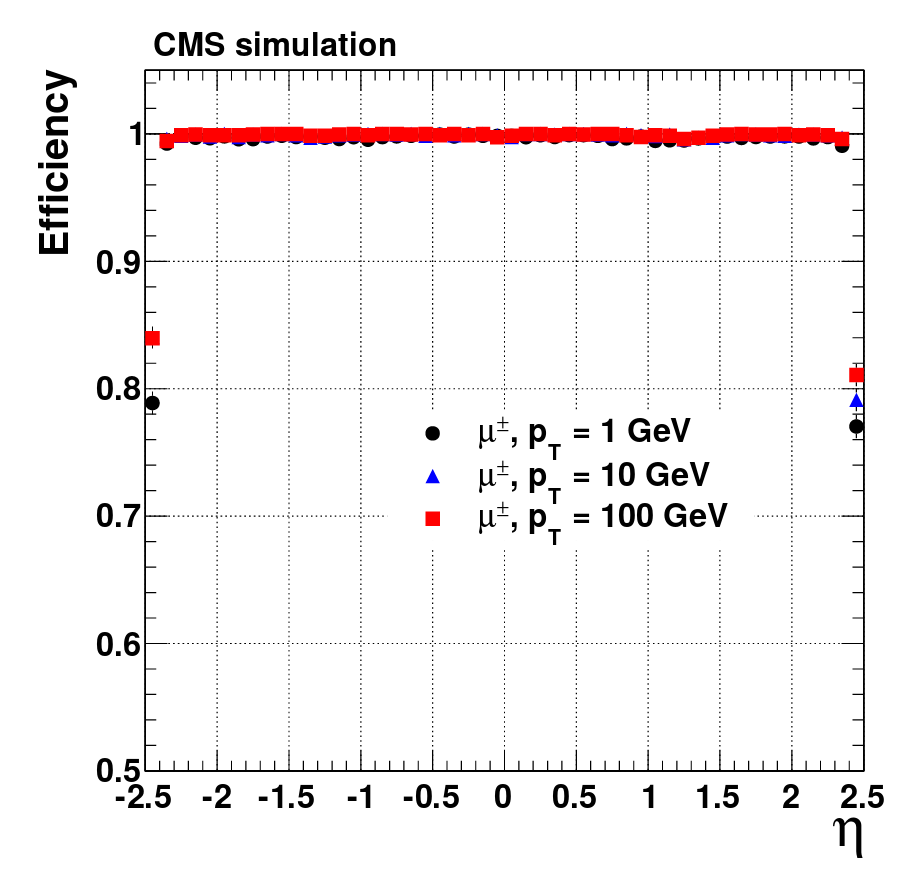
\includegraphics[width=.4\textwidth]{muon_eff_eta}\hspace{1cm}
 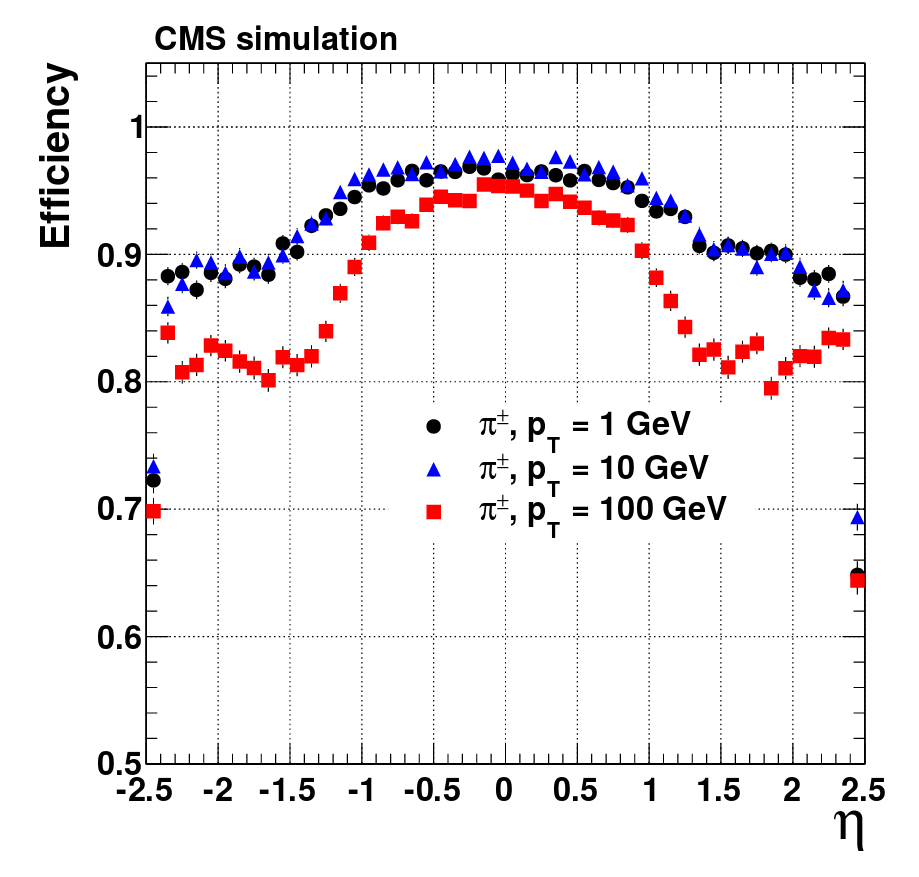
\includegraphics[width=.4\textwidth]{pion_eff_eta} 
 \caption{The muon efficiency (left) and pion efficiency (right) as a function of pseudorapidity, for multiple transverse momenta.~\cite{Chatrchyan:2014fea}}
 \label{fig:eff_eta}
\end{figure}

Finally, the primary vertex is reconstructed from the tracks. Since the collisions happen between bunches of protons, multiple protons will be colliding at the same time. The extra collisions, next to the potentially interesting collision, are referred to as pile-up interactions. The particles generated in these collisions are all detected simultaneously and form a challenge to disentangle them from the particles coming from the to be studied interaction.

The reconstruction is done in 2 steps: first the tracks that appear to originate from the same interaction vertex are clustered, then a fitting procedure computes the vertex parameters and assigns a weight to each associated track, reflecting the probability that it corresponds to the considered vertex. Figure~\ref{fig:PV} shows the reconstruction efficiency and the resolution of the primary vertex. The more tracks, the better the vertex is constrained and thus the better the resolution.

\begin{figure}[ht]
  \centering
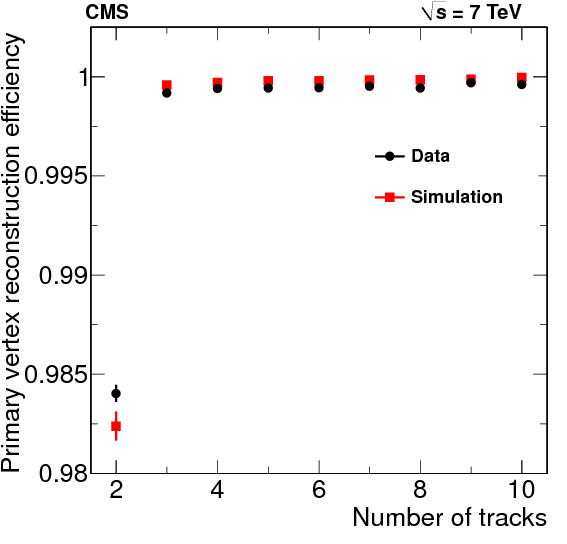
\includegraphics[width=.4\textwidth]{PV_eff}\hspace{1cm}
 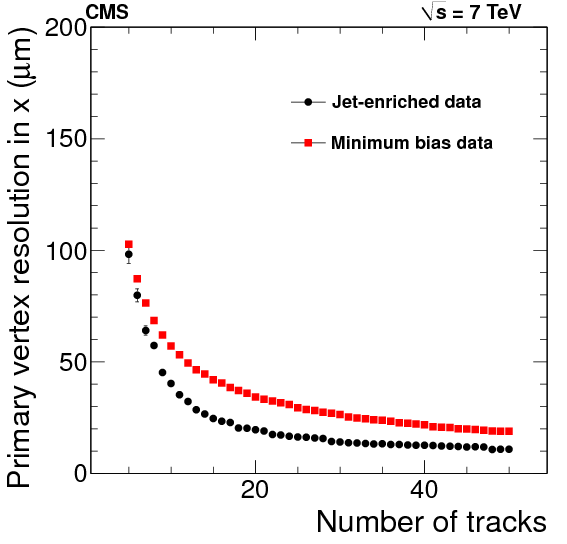
\includegraphics[width=.4\textwidth]{PV_res} 
 \caption{The primary vertex reconstruction efficiency (left) and resolution (right) as a function of the number of tracks associated to it.~\cite{Chatrchyan:2014fea}}
 \label{fig:PV}
\end{figure}

\subsection{Electron and isolated photon reconstruction}
\label{sec:electron_reconstruction}

Electrons are reconstructed using information from both the tracker and the calorimeters. Due to the large amount of material present in the tracker, electrons will emit bremsstrahlung photons, and photons will often convert into $e^+e^-$ pairs, which can again radiate bremsstrahlung photons. The electron and photon reconstruction is therefore very similar.

For electrons, a \ac{GSF}~\cite{} candidate is taken as starting point. This candidate is obtained using 2 different methods to reconstruct the electron track from the hits in the tracker. This track reconstruction should gather all radiated energy from the electron. First, the ECAL-based approach is used, grouping \ac{ECAL} clusters into superclusters. These superclusters collect the energy of the electron and the bremsstrahlung photons in a small $\eta$ window and a large $\phi$ window, taking the bending of the electron track in the magnetic field into account. The supercluster energy and position is then used to determine the position of the corresponding hits in the tracker layers. Next, the tracker-based approach is used to reconstruct electrons missed by the ECAL-based method. In this case, all the tracks from the iterative tracking with transverse momentum larger than \SI{2}{GeV} are used. The obtained electron seeds are then used in the specific electron tracking, done by a \ac{GSF} fit, which is more adapted to electrons than the Kalman filter used in the iterative tracking, as it describes the energy loss in each tracker layer. In the case of isolated photons, a candidate is seeded from an \ac{ECAL} supercluster with transverse energy larger than \SI{10}{GeV} which is not linked to a \ac{GSF} track.

The total energy of the accumulated \ac{ECAL} clusters is corrected for the energy that was lost in the process, using analytical functions of the energy and pseudorapidity. The applied corrections can be as large as 25\%, at low transverse momentum and at $|\eta| = 1.5$, where the material density in the tracker is largest. The energy of the electron is then obtained from a combination of the corrected energy and the momentum of the \ac{GSF} track, while the direction of the electron is taken from the \ac{GSF} track. For photons, the corrected energy and the direction of the supercluster are used.

Additionally, the electron and photon candidates must satisfy identification criteria to be retained. In the case of electrons a boosted decision tree is used, combining fourteen variables including the amount of energy radiated and the ratio between the energies gathered in HCAL and ECAL, while for photons the candidates must be isolated from other tracks and calorimeter clusters, and the energy distribution in the \ac{ECAL} and the ratio between the \ac{HCAL} and \ac{ECAL} energies must be compatible with the expectation from a photon shower.

\subsection{Muon reconstruction}
\label{sec:muon_reconstruction}

Muon tracking is performed using 2 complementary approaches. The first method starts from standalone muons which are reconstructed from hits in the muon detectors using pattern recognition. The standalone muons are then matched to tracks in the tracker, and the hits are combined to form a global muon track. This global muon fit improves the momentum resolution compared to the tracker-only fit at muon momenta larger than \SI{200}{GeV}.

For momenta below \SI{10}{GeV}, muons often fail the global muon conditions which require the muon to penetrate through more than one muon detector plane, due to the large multiple scattering in the return yoke. In this case, tracker muon reconstruction is more efficient since it only requires one muon segment. Each track in the tracker with a transverse momentum larger than \SI{0.5}{GeV} and a total momentum larger than \SI{2.5}{GeV} is therefore extrapolated to the muon system and if at least one matching track segment is found, it is retained as muon candidate.

Within the geometrical acceptance of the muon system about 99\% of the muons are reconstructed, either as global muon or as tracker muon and frequently as both. Global and tracker muons that share the same track inside the tracker are merged into a single candidate. Muons that are only reconstructed as standalone muons have a worse momentum resolution compared to the global and tracker muons.

Charged hadrons can be misreconstructed as muons if e.g. a part of the hadron shower reaches the muon system. In order to improve the muon identification, the \ac{PF} muon identification algorithm described in Section~\ref{sec:PF} also matches energy deposits in the \ac{ECAL} and \ac{HCAL} with the muon track.

\subsection{Particle flow}
\label{sec:PF}

The \acf{PF} algorithm reconstructs so-called particle flow candidates by combining information from all different \ac{CMS} subdetectors, linking different elements, such as tracks in the tracker, calorimeter clusters, and muon tracks. The obtained collection of particle candidates is subsequently used to reconstruct jets and to determine the missing transverse energy.

In a first step, the \ac{PF} algorithm identifies charged particle tracks, as defined in Section~\ref{sec:tracking}, and Sections~\ref{sec:electron_reconstruction} and \ref{sec:muon_reconstruction} for electron and muon tracks, respectively. At the same time, the calorimeter clusters are reconstructed with a clustering algorithm designed specifically for the \ac{PF} event reconstruction. In this algorithm, cluster seeds are first identified as local energy maxima above a given seed threshold, and with respect to the four or eight closest cells. The clusters are then formed by accumulating neighboring cells with an energy above a given cell threshold, in order to suppress noise.

The \ac{PF} elements in the different subdetectors are then connected by a link algorithm which avoids any double counting. The link algorithm produces blocks of associated elements, quantifying the quality of the link by defining a distance between the elements. When an element is linked to multiple other elements, only the link with the shortest distance is kept. More precisely, a link between a track in the tracker and a calorimeter cluster is made by extrapolating it from the last hit in the tracker to the calorimeters. The distance between the position of the extrapolated track and the cluster in the ($\eta$, $\phi$) plane is then used to define the link distance. At the interaction points between the track and the tracker layers, tangents to the \ac{GSF} tracks are extrapolated to the \ac{ECAL} in order to collect the energy of photons radiated by electron bremsstrahlung. A dedicated conversion finder was also developed to identify bremsstrahlung and prompt photon conversions into $e^+e^-$ pairs. Links between calorimeter clusters are established outside of the tracker acceptance, or between the preshower and \ac{ECAL} clusters in the preshower acceptance. In this case the link distance is also defined as the distance between the position of the clusters. Charged particle tracks can also be linked by a common secondary vertex. Finally, links between tracks in the tracker and in the muon detectors are established as explained in Section~\ref{sec:muon_reconstruction}.

In a next step, the \ac{PF} blocks are classified as muons, electrons, or isolated photons. The corresponding elements are then excluded from further consideration. Once electrons, muons, and isolated photons have been identified, the remaining elements are identified as charged hadrons, neutral hadrons, or photons produced in jets. Within the tracker acceptance, the \ac{ECAL} clusters not linked to any track are classified as photons, while the clusters in the \ac{HCAL} without a matched track are labeled as neutral hadrons. Outside of the tracker acceptance, charged and neutral hadrons can not be distinguished. \ac{ECAL} clusters linked to an \ac{HCAL} cluster are then assumed to arise from the same hadron shower, and the estimated energy for these particles is the sum of the energy deposited in the \ac{ECAL} and the \ac{HCAL}. The remaining clusters are then linked to one or several tracks in order to reconstruct the charged hadrons.

\subsection{Jet reconstruction}
\label{sec:jet_reconstruction}

Jets are reconstructed with the anti-$k_T$ algorithm~\cite{1126-6708-2008-04-063}, which clusters either the particles reconstructed by the \ac{PF} algorithm (\ac{PF} jets) or the energy deposits in the calorimeters (Calo jets). This procedure takes into account the transverse momentum $p_T$, also called $k_T$, of the particles and the distance between particles, defined as \begin{equation}                                                                                                                                                                                                                                                                                                     
 \Delta R_{ij} = \sqrt{(y_i - y_j)^2 + (\phi_i - \phi_j)^2}.                                                                                                                                                                                                                                                                                        \end{equation}
The strategy consists of the following steps:
\begin{enumerate}
 \item For every pair of particles $i$ and $j$, a distance $d_{ij}$ defined as 
 \begin{equation}
  d_{ij} = \min\left(\frac{1}{p_{Ti}^2}, \frac{1}{p_{Tj}^2} \right)\frac{\Delta R_{ij}^2}{R^2}
 \end{equation}
 is calculated.
 \item For every particle $i$, a distance $d_{iB}$ to the beam pipe is calculated with
 \begin{equation}
  d_{iB} = 1/p_{Ti}^{2}.
 \end{equation}
 \item The minimum of $d_{ij}$ and $d_{iB}$ is then determined.
 \item If it is $d_{ij}$, particles $i$ and $j$ are recombined into a new particle by adding the four-momenta of the particles. If it is $d_{iB}$, particle $i$ is declared to be a jet and it is removed from the list of particles.
 \item This is repeated until no particles remain.
\end{enumerate}

In this clustering algorithm, the parameter $R$ determines what is called a jet. If a particle $i$ has no other particles within a distance $R$, $d_{iB}$ will be smaller than $d_{ij}$ and the particle will become a jet. A consequence of this is that an arbitrarily soft particle can become a jet, and therefore a minimum transverse momentum for a jet to be of interest is defined.

The anti-$k_T$ algorithm favors clustering around hard particles, and the jets then grows outward from this seed. However, since it still involves a combination of energy and angle in the distance measure, this is a collinear-safe growth, meaning that the jet will not change when one of the particles of the jet is split collinearly. This algorithm is also infrared-safe, i.e. the same set of jets is obtained when soft particles are emitted. and gives rise to circular jets.

A reliable determination of the jet energy is however not straightforward, since many effects can distort the energy estimation, such as the calorimeter response, the limited particle reconstruction efficiency, the underlying event, the pileup, and the charged particles bending out of the jet cone due to the strong magnetic field. The pileup is mitigated by applying \ac{CHS}, which consists of removing charged hadrons associated with vertices other than the primary vertex from the list of \ac{PF} candidates. Additionally, the jet energy is corrected using a factorized approach with the following steps:
\begin{itemize}
 \item \textbf{Pileup correction (L1).} The first level of jet energy corrections is applied event-by-event and jet-by-jet, and is determined from simulation. It is dependent on the pseudorapidity and transverse momentum of the jet, the average $p_T$ density in the event, and the effective jet area. This effective area is determined by injecting a large number of very soft particles in the event before the jet clustering. The spread of the soft particles in each jet then defines the jet area.
 \item \textbf{Relative $\eta$ and absolute $p_T$ corrections (L2L3).} This correction is also obtained from simulations and corrects for the non-uniform response of the calorimeters in $\eta$ and $p_T$. 
 \item \textbf{Residual $\eta$ and $p_T$ corrections (L2L3Residual).} Since the L2L3 correction is derived from simulation, additional residual corrections are needed.
\end{itemize}

Finally, a set of identification criteria are applied on the \ac{PF} jets. A jet is required to consist of at least two particles. For jets in the region $|\eta| < 2.7$, the fraction of energy coming from ether neutral hadrons or photons should not exceed 99\%. Additionally, for jets restricted to the tracker acceptance ($|\eta| < 2.4$), there should at least be some energy deposited in the \ac{HCAL}, the jet should contain 1 or more charged constituent, and the fraction of energy corresponding to electrons or photons should not exceed 99\%.

\subsection{Missing transverse energy reconstruction}

While most particles produced in the collisions can be reconstructed from the hits and energy deposits in the detector, neutrinos are neutral and weakly interacting and will therefore traverse the entire detector, escaping detection. Other hypothetical neutral weakly interacting particles, which are being searched for in many physics analyses, would escape the detector without producing hits as well. This makes an accurate reconstruction of this type of particles rather challenging.

In order to be able to reconstruct neutrinos and search for new neutral and weakly interacting particles, another method is used, based on indirect observations. As the detector is hermetically closed such that all other particles in the event can be detected, the missing transverse energy can be determined. This energy then corresponds to all neutrinos and other weakly interacting neutral particles in the event, and can be calculated from the total transverse momentum of all the observed final state particles as 
\begin{equation}
 \vec{E}_T^{miss} = - \sum \vec{p}_T,
\end{equation}
where the sum runs over all reconstructed \ac{PF} particles.

\section{Simulation of the SIMP signal}
\label{sec:SIMPs}

For the generation of the \ac{SIMP} signal, the model Lagrangian given in equation~\ref{} is implemented in \textsc{FeynRules 2.0}~\cite{Alloul:2013bka}. Next, the matrix element is calculated at \ac{LO} and events are generated using \textsc{Madgraph 5}. The subsequent parton shower and hadronization is done with \textsc{Pythia 8}, using tune CUEP8M1. Next, the events are simulated in the \ac{CMS} detector using \textsc{Geant}. However, the \acp{SIMP} are not included in the simulation, as their interaction with matter is not implemented in \textsc{Geant}. The \acp{SIMP} were instead incorporated by adding an additional step to the standard reconstruction described in Section~\ref{sec:reconstruction}. In this additional step the \acp{SIMP} are directly converted to neutral \ac{PF} candidates and merged with the rest of the \ac{PF} candidates. The standard pileup corrections, jet clustering, and charged hadron subtraction are then applied in order to obtain the resulting jets, denoted here as P2PF jets.

In order to validate this method, a second sample was produced using neutrons instead of \acp{SIMP} and applying the same additional step. In this case the the neutrons will also be correctly reconstructed by the standard reconstruction. The reconstructed \ac{PF} candidates that are matched to the generated neutrons were therefore removed before injecting the converted generated neutrons to the collection of \ac{PF} candidates. This sample is then used to evaluate the difference with a standard neutron sample where the full \textsc{Geant} simulation is done. Neutrons were chosen because of their resemblance to the \acp{SIMP} as single neutral particles generating a hadronic shower.

The two leading generator-level jets (GEN) can then be compared to the uncorrected P2PF jets from the custom sample and the \ac{PF} jets from the standard sample. The transverse momentum of these jets is compared in Figure~\ref{fig:neutron}. This shows that the \ac{JER} is not described properly, since the additional step directly converts generated particles to \ac{PF} candidates without taking into account any other effects. In order to produce a more realistic simulation, the new \ac{PF} candidates are therefore smeared with \ac{JER} distributions derived using the uncorrected \ac{PF} jets matching the neutrons in the standard neutron sample in bins of $\eta$ and $p_T$. An example of this resolution is shown in Figure~\ref{fig:neutron_res} for central neutrons with low and high transverse momentum.

\begin{figure}[ht]
  \centering
 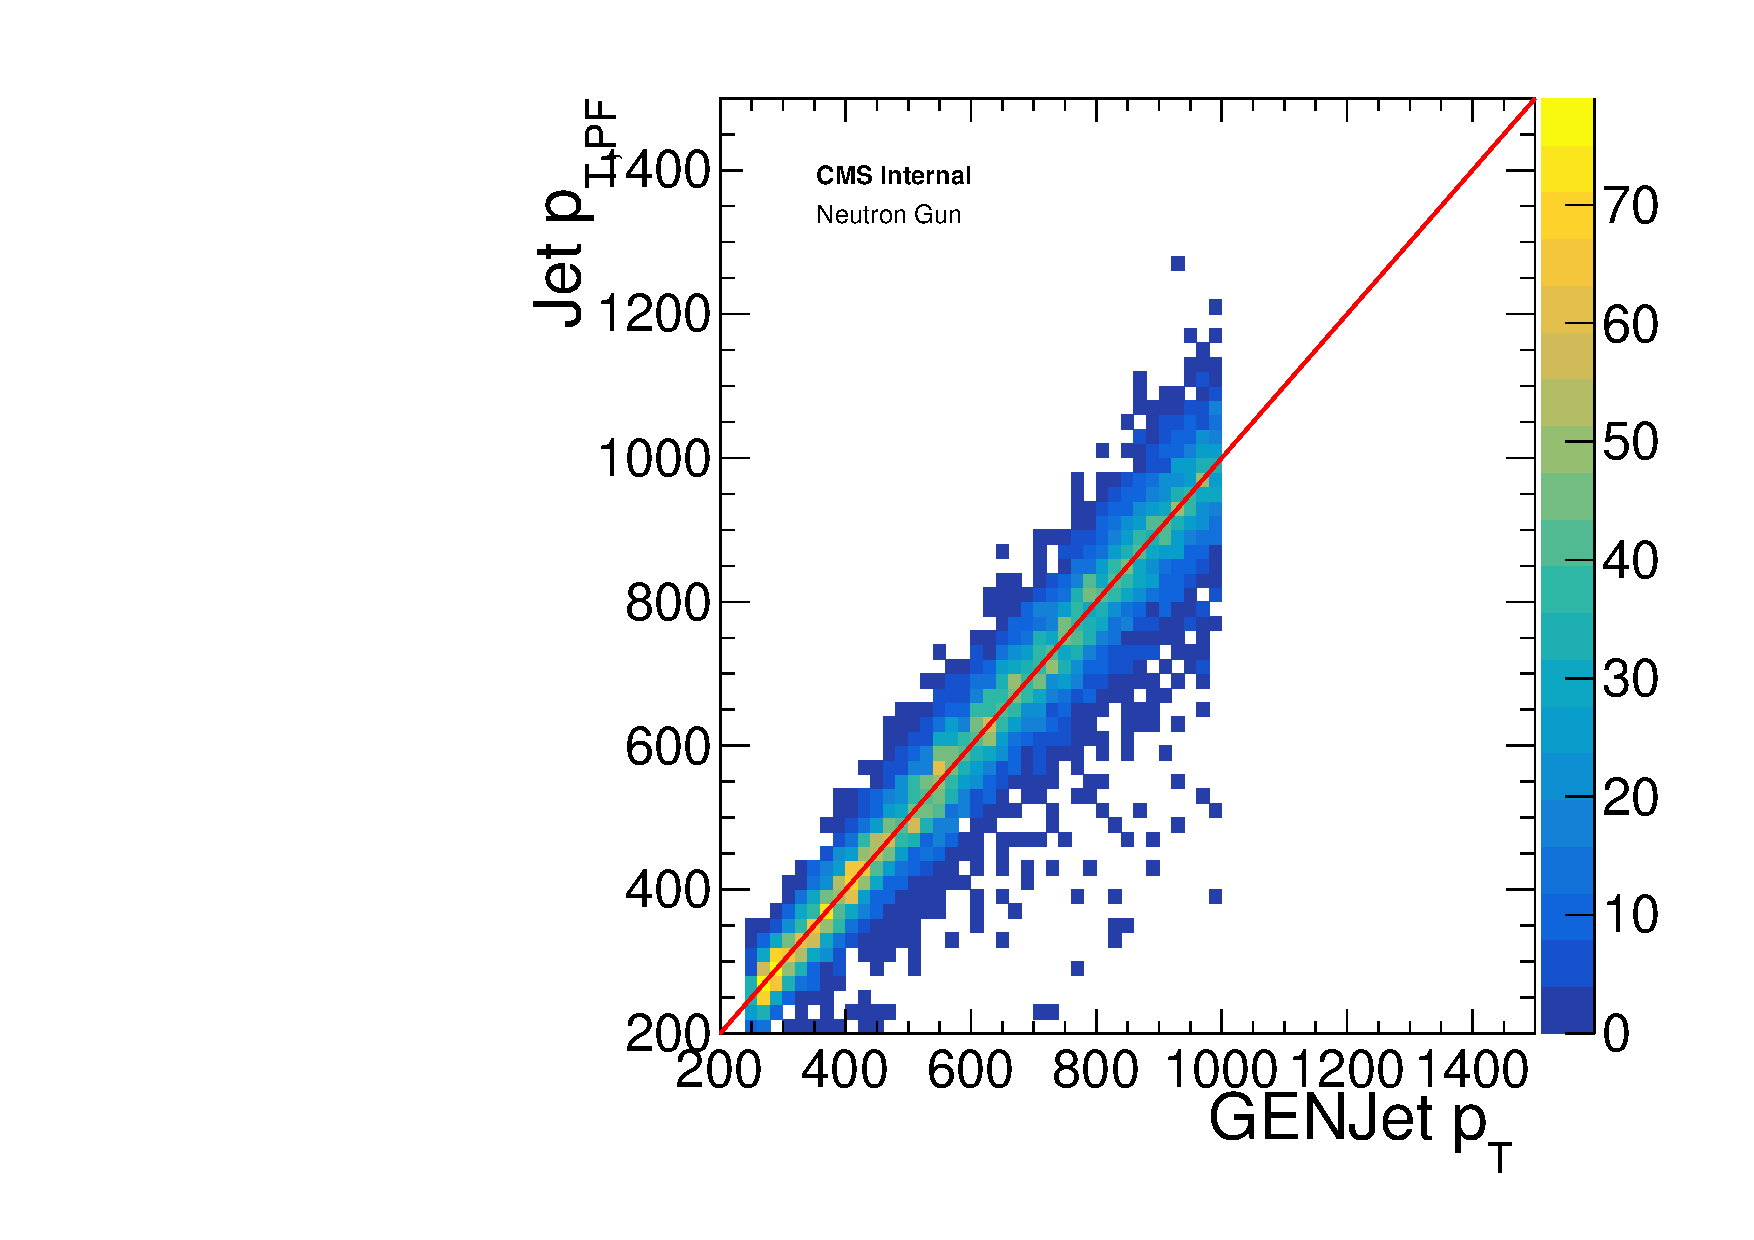
\includegraphics[width=.48\textwidth]{pt_neutron_gun_th2f_JECs_GetRandom2.pdf} \hfill
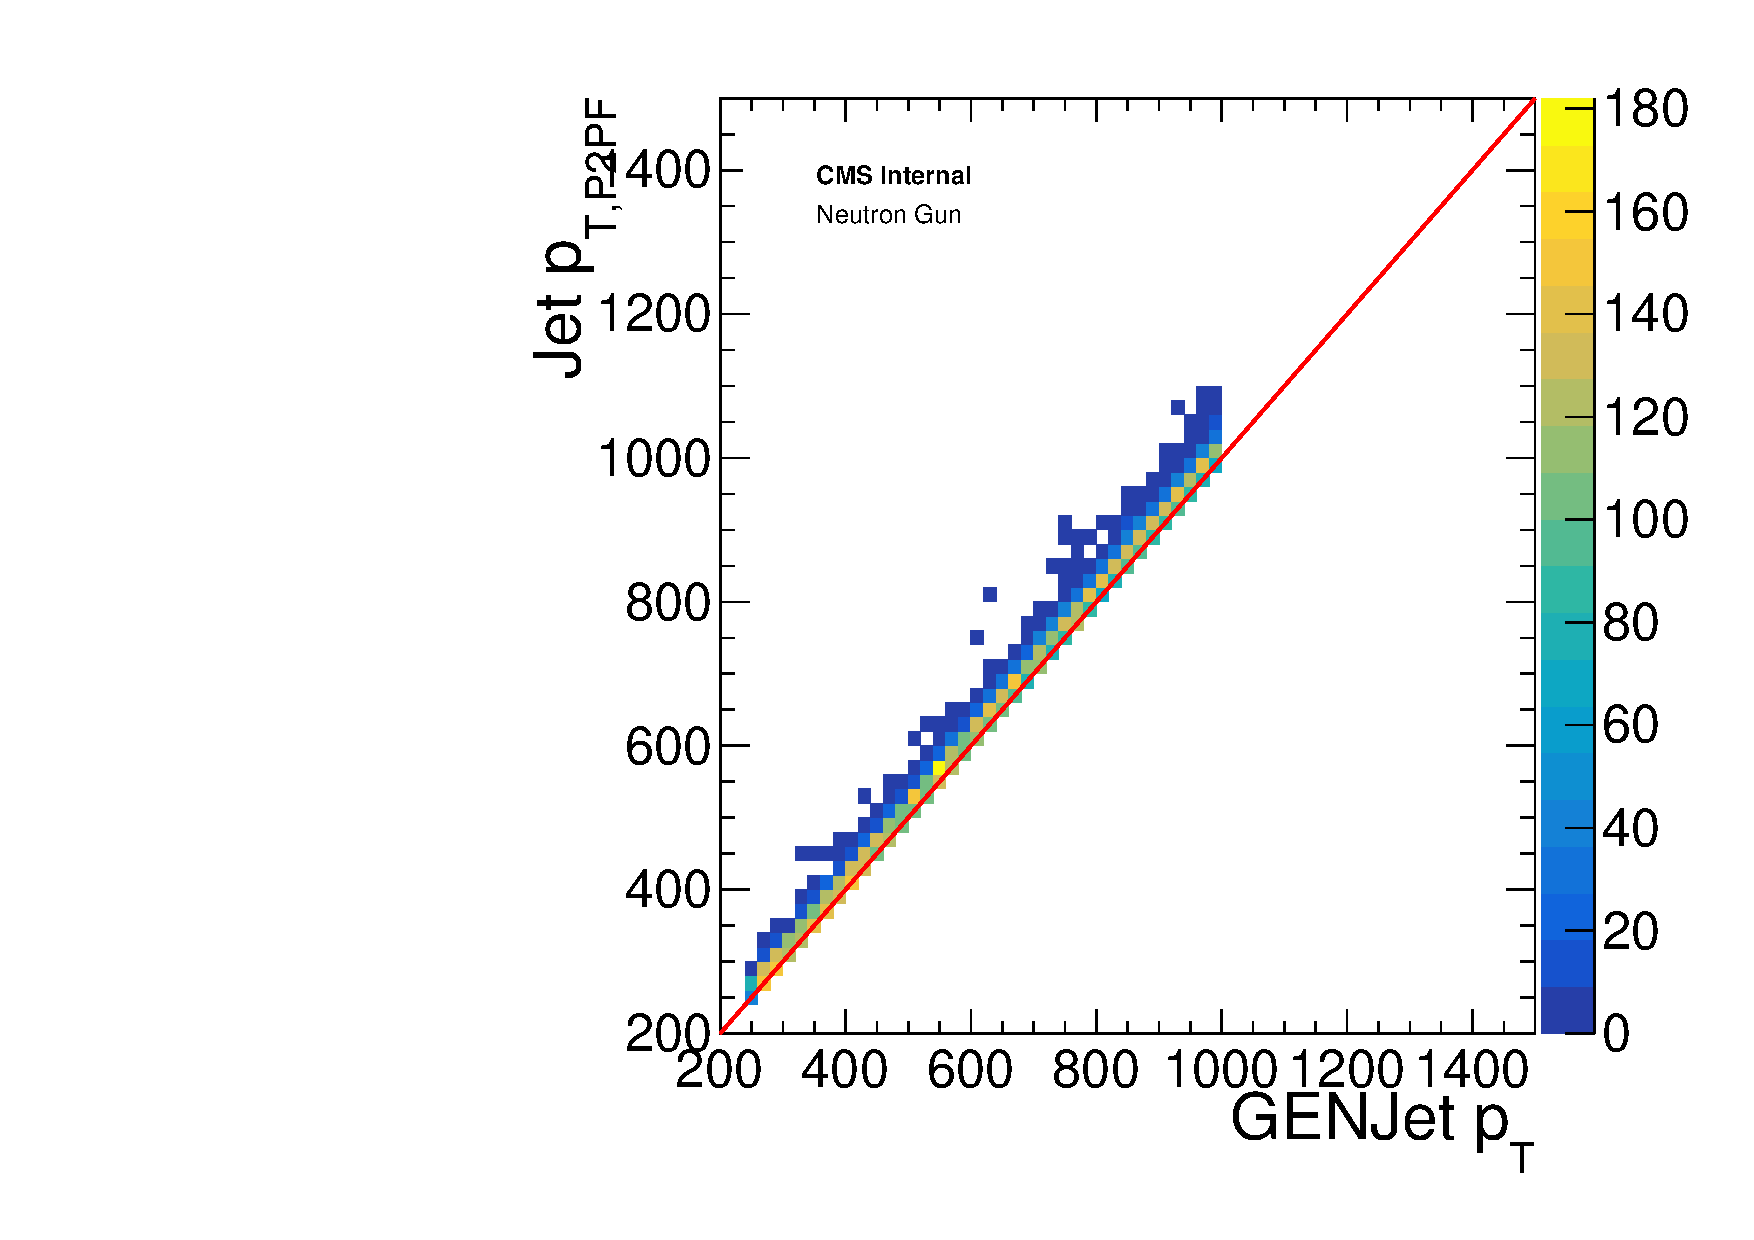
\includegraphics[width=.48\textwidth]{pt_neutron_gun_p2pf_th2f_NoSmearing.pdf}
 \caption{Comparison of the transverse momentum of the generator-level jets to the \ac{PF} jets (left) and P2PF jets (right) without jet energy resolution smearing, using a neutron sample.}
 \label{fig:neutron}
\end{figure}

\begin{figure}[ht]
  \centering
 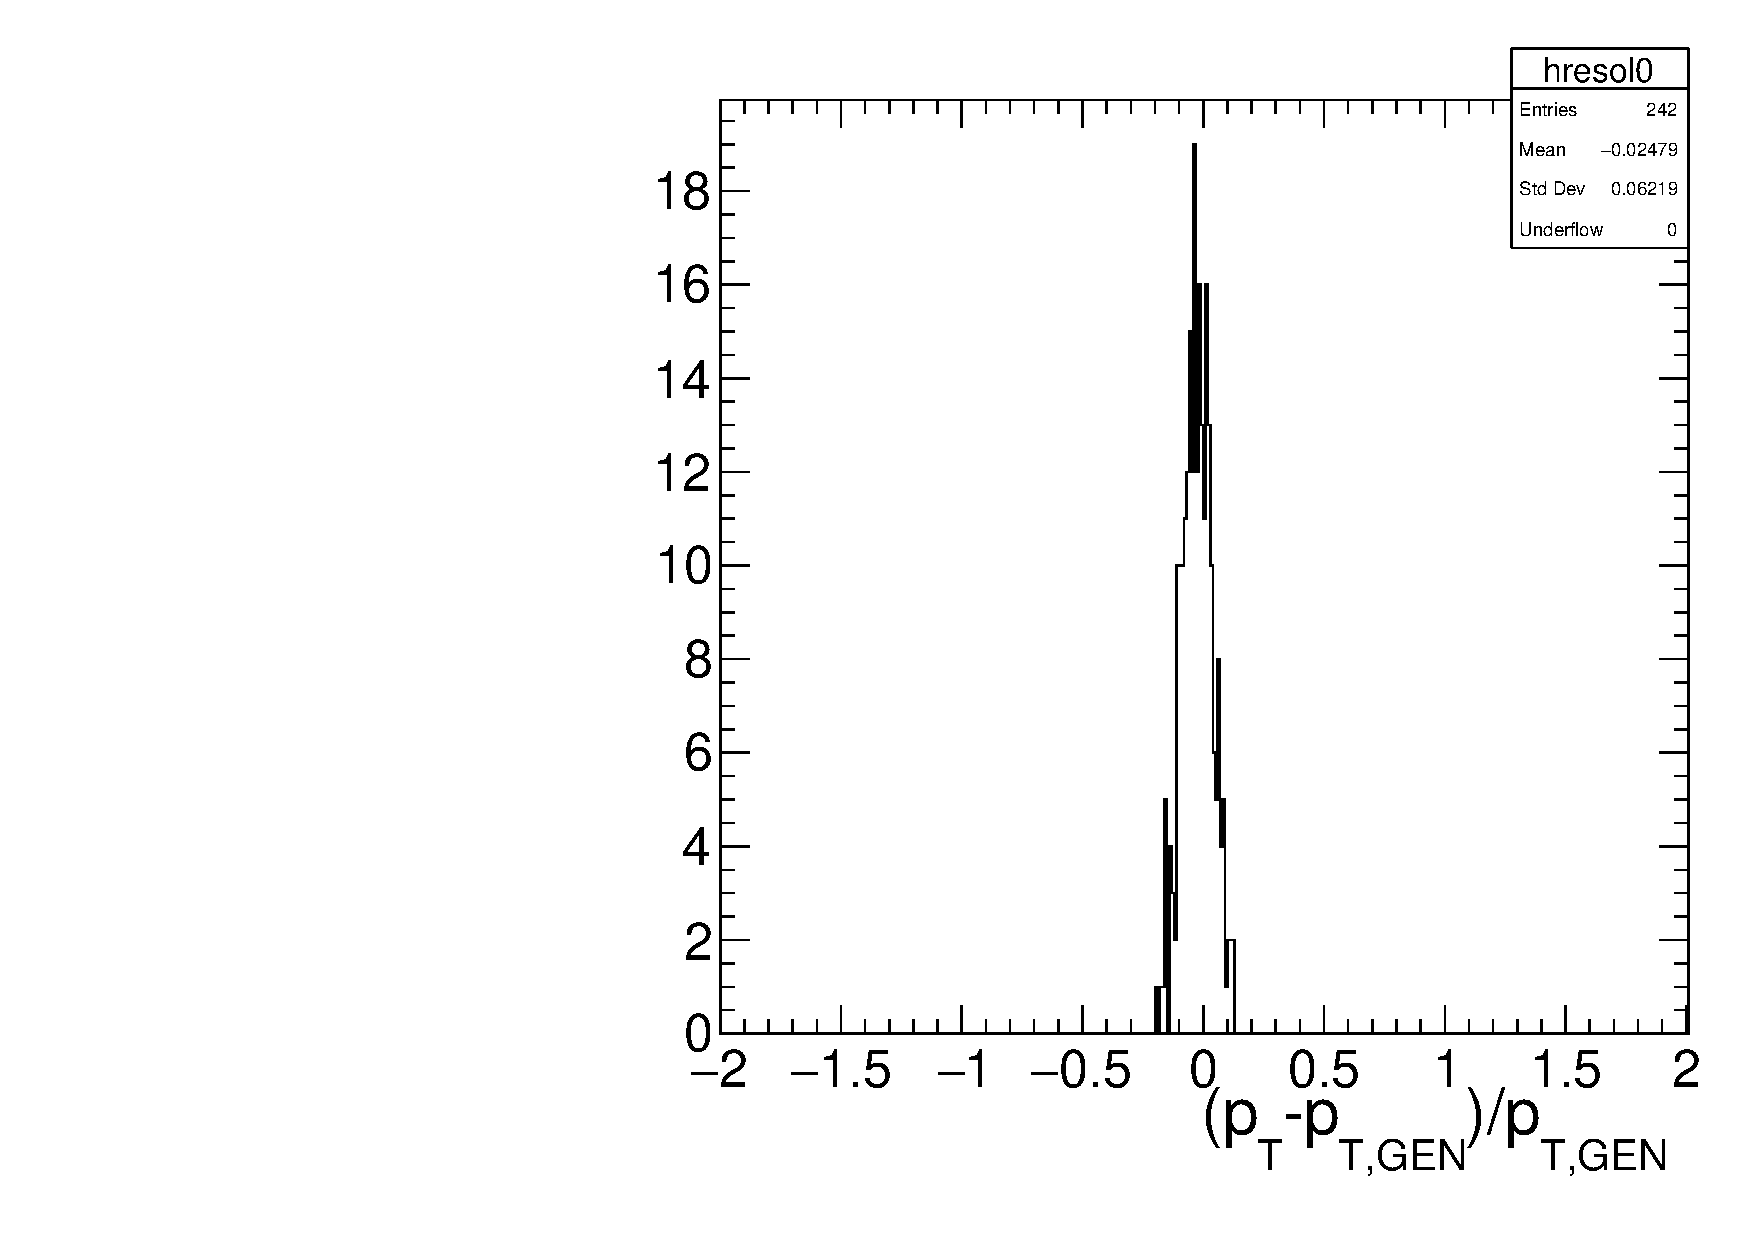
\includegraphics[width=.48\textwidth]{pt_res_ptbin_0.pdf} \hfill
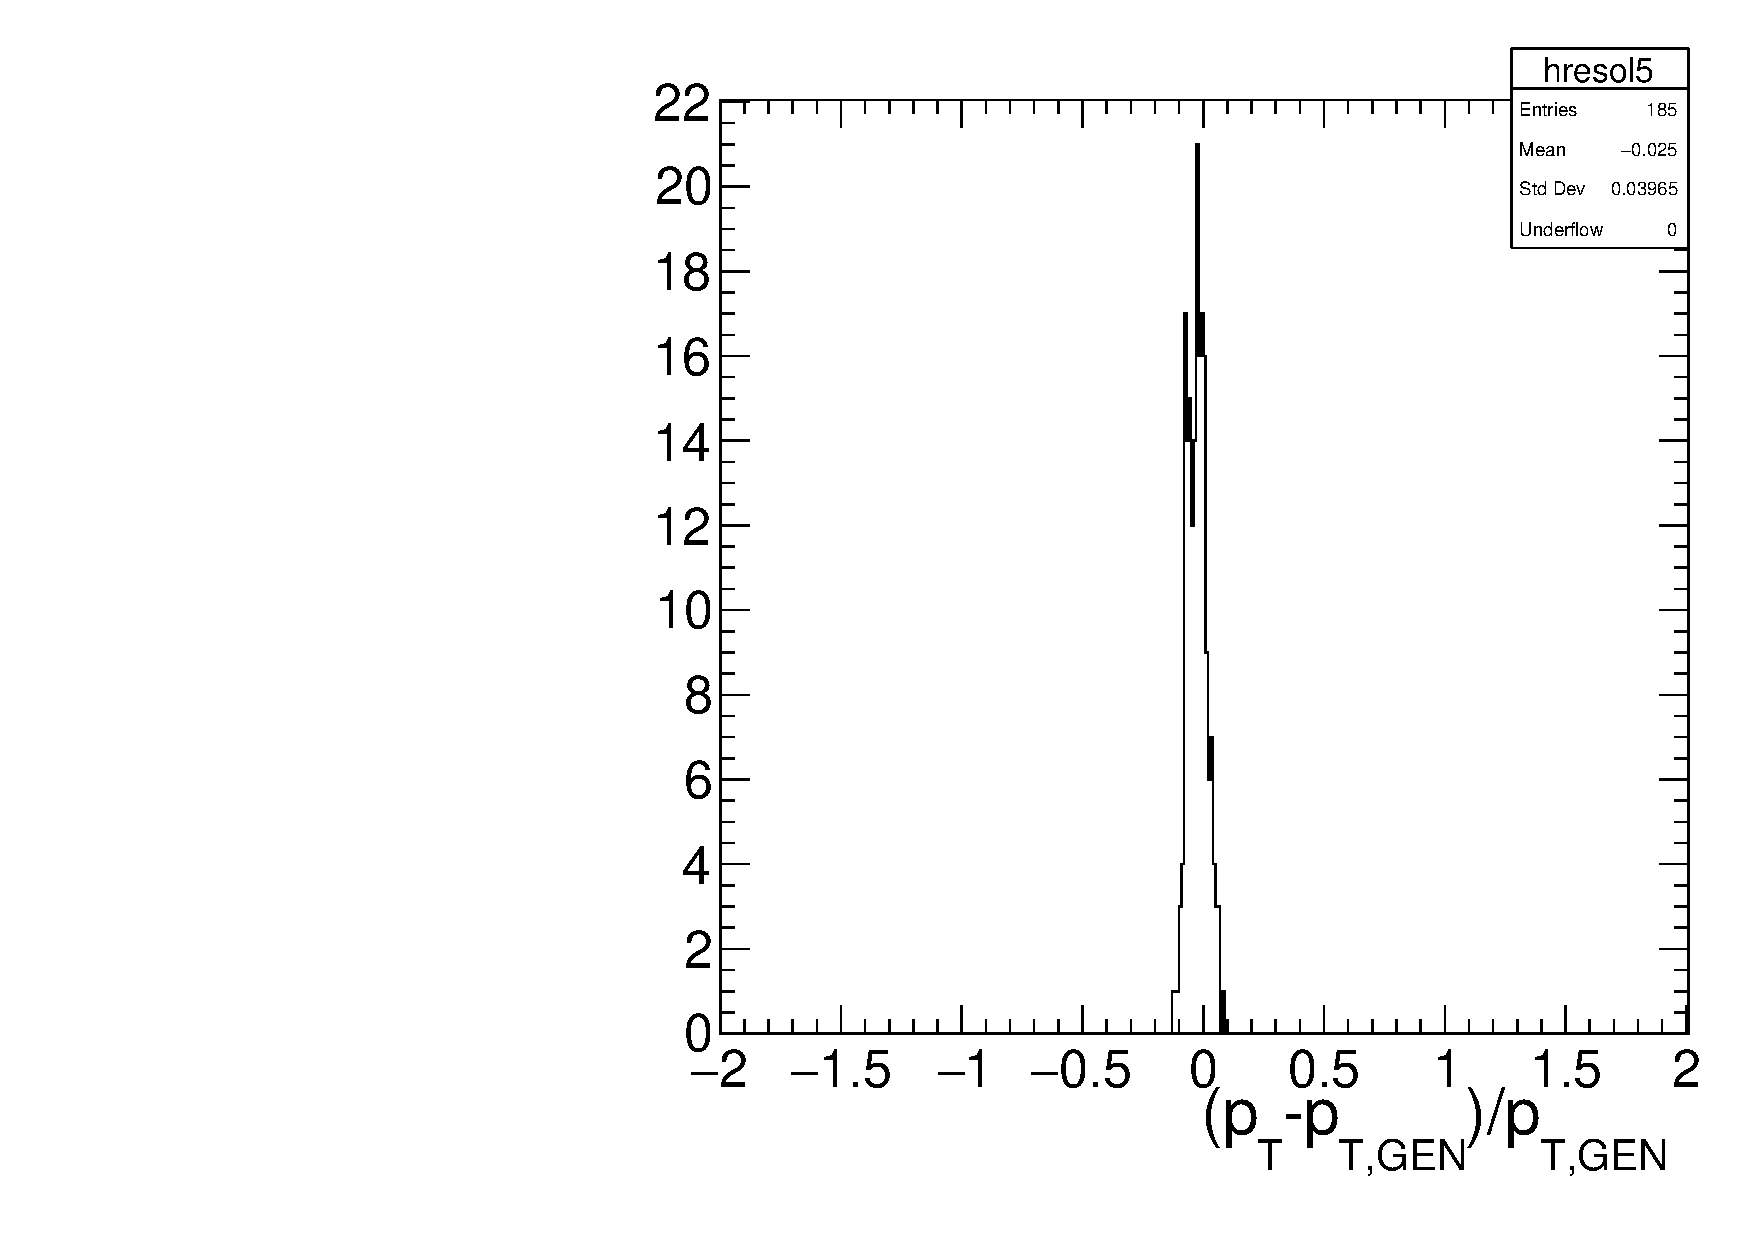
\includegraphics[width=.48\textwidth]{pt_res_ptbin_5.pdf}
 \caption{The jet energy resolution of neutrons with $0< |\eta| < 0.5$ and \SI{200}{GeV}$<p_T<$\SI{300}{GeV} (left) or \SI{700}{GeV}$<p_T<$\SI{800}{GeV} (right).}
 \label{fig:neutron_res}
\end{figure}

After applying this smearing, the P2PF jets are processed with the standard sequence of charged hadron subtraction, jet clustering, L1FastJet, and L2/L3 corrections. The comparison of the corrected P2PF jets and the standard corrected \ac{PF} jets is shown in Figure~\ref{fig:neutron_corr} for the neutron sample, validating that the jet transverse momentum is now correctly smeared. The \ac{JER} distributions are also compared in Figure~\ref{fig:neutron_res_corr} and fitted with a Crystal Ball function, showing compatible parameters. This demonstrates that the procedure, where the \ac{JER} distributions derived from a neutron sample are used to smear the \ac{PF} candidates from generator-level \acp{SIMP}, can sufficiently accurately simulate \acp{SIMP} in a realistic detector.

\begin{figure}[ht]
  \centering
 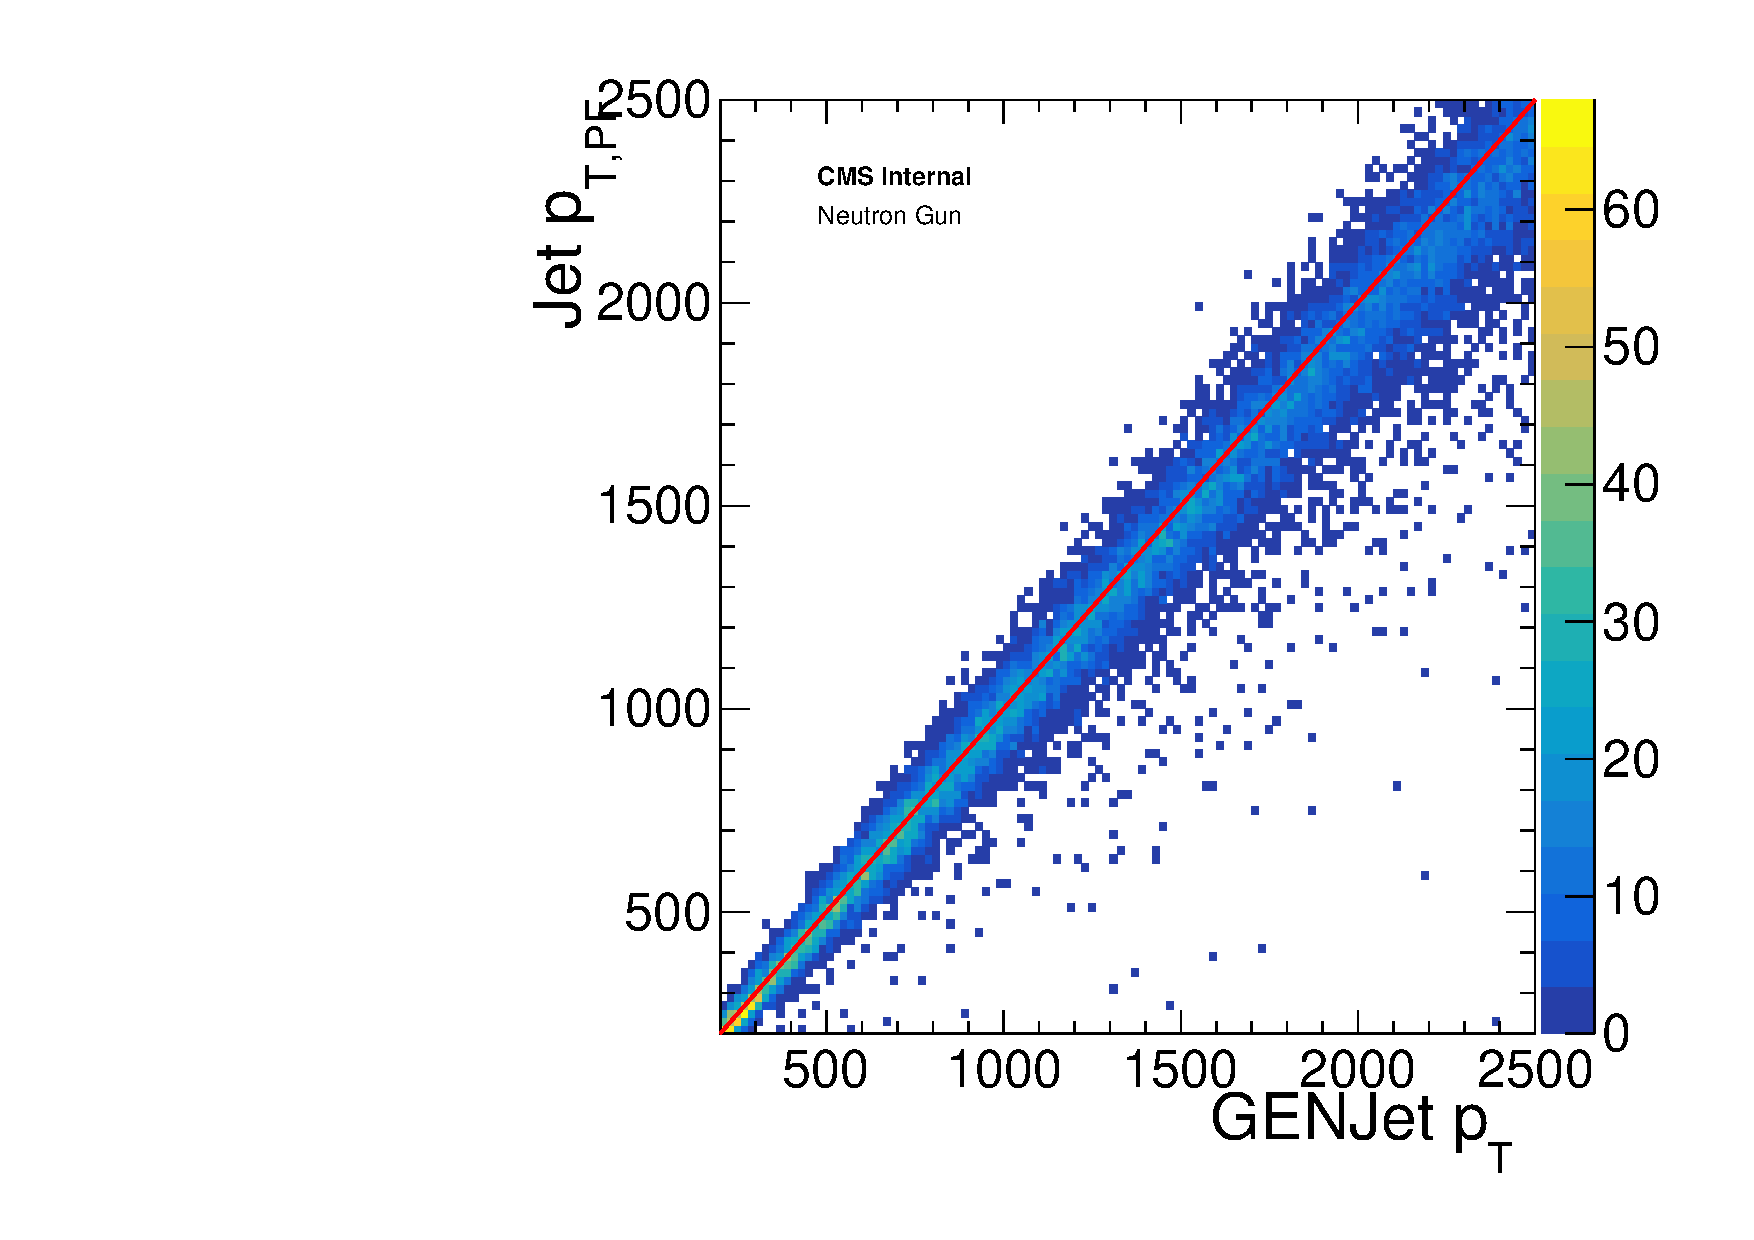
\includegraphics[width=.48\textwidth]{pt_neutron_gun_th2f_005.pdf} \hfill
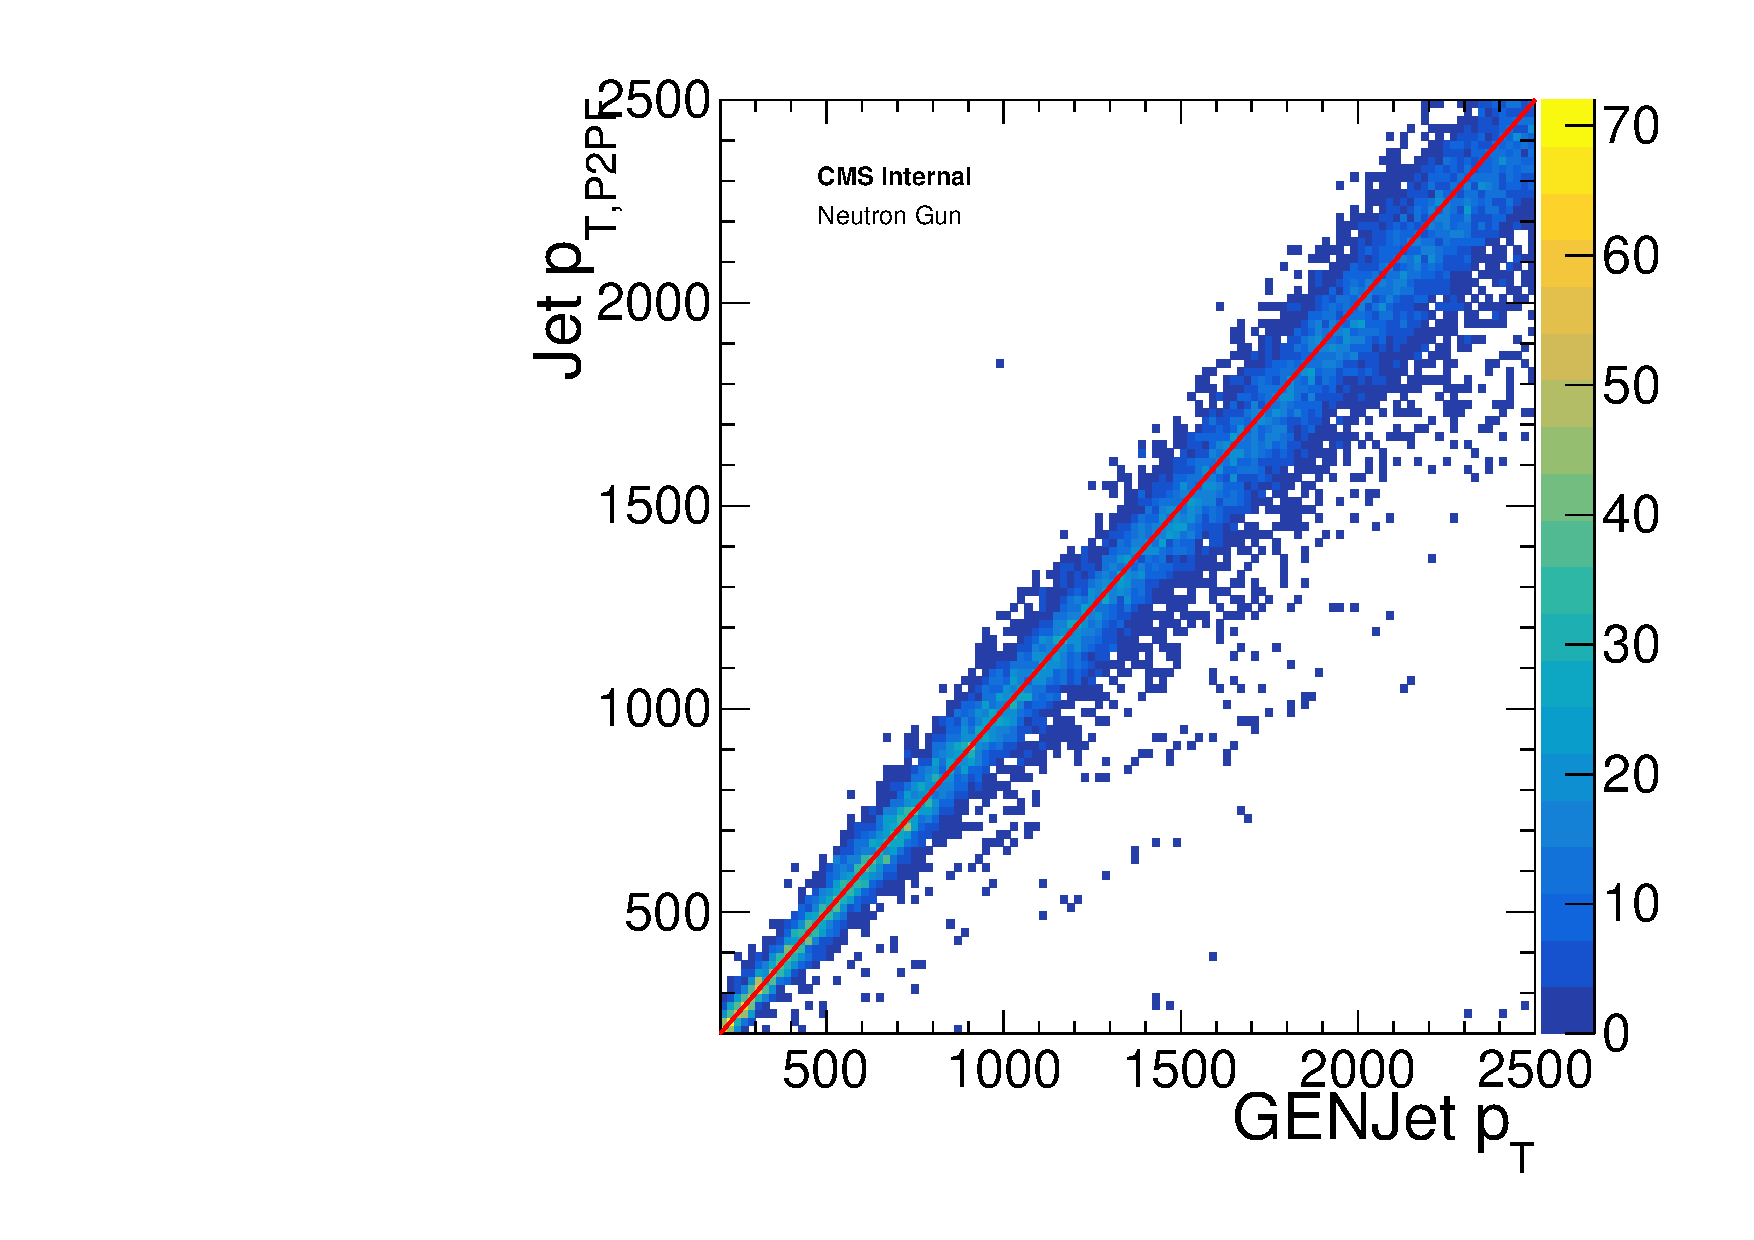
\includegraphics[width=.48\textwidth]{pt_neutron_gun_p2pf_th2f_005.pdf}
 \caption{Comparison of the transverse momentum of the generator-level jets to the \ac{PF} jets (left) and P2PF jets (right) in the region $0< |\eta| < 0.5$ with jet energy resolution smearing, using a neutron sample.}
 \label{fig:neutron_corr}
\end{figure}

\begin{figure}[ht]
  \centering
 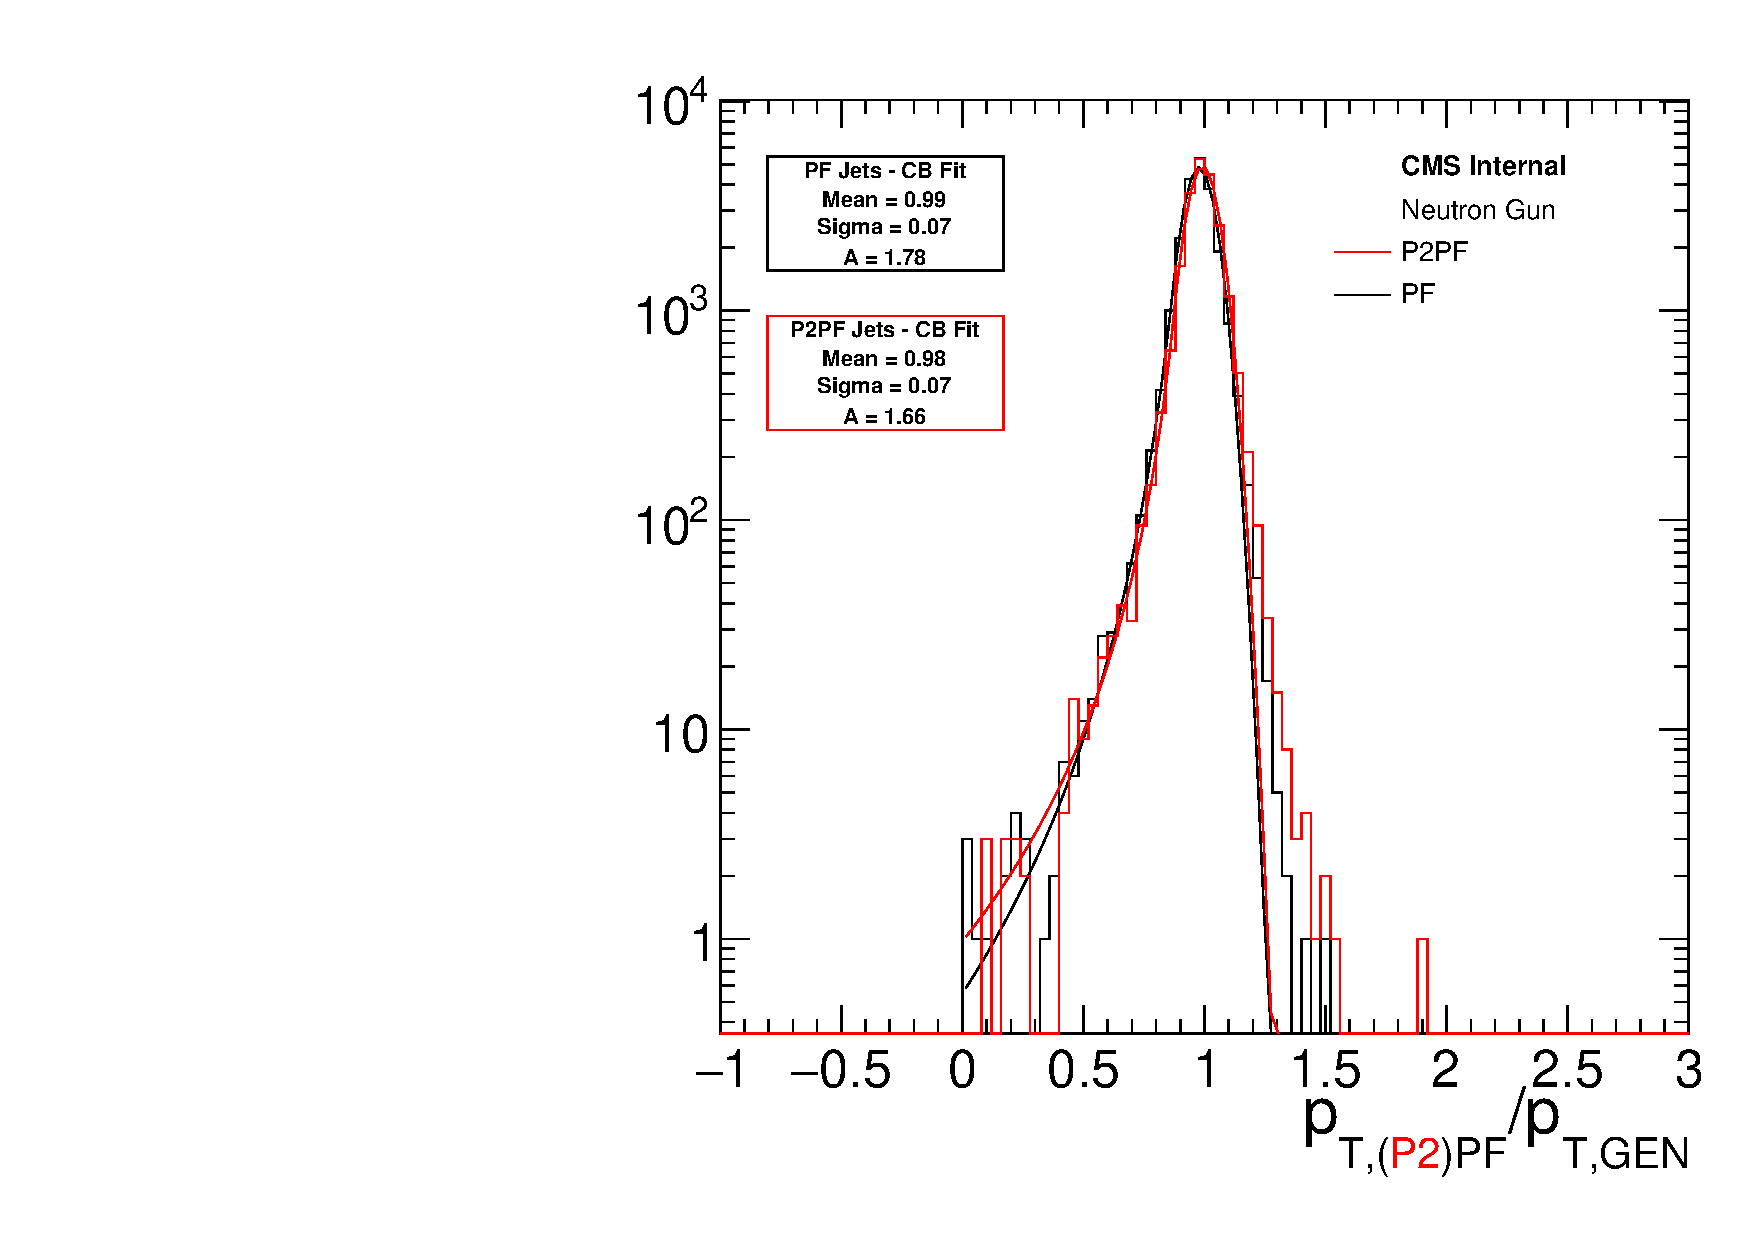
\includegraphics[width=.75\textwidth]{pt_neutron_gun_res_fit_005.pdf} 
 \caption{The jet energy resolution of the corrected P2PF jets (red) and \ac{PF} jets (black), fitted with a Crystal Ball function.}
 \label{fig:neutron_res_corr}
\end{figure}

\clearpage
\clearpage{\pagestyle{empty}\cleardoublepage}
